\section{Method}
\label{sec:method}

The chain is: Euler wave drag of each nose $\rightarrow$ vehicle drag build-up $\rightarrow$ ascent
trajectory $\rightarrow$ apogee, heating, stability. All scripts are in \texttt{scripts/} (Appendix~\ref{app:scripts}).

\subsection{Nose wave drag: axisymmetric Euler solver}
\label{sec:euler}

Above Mach 1 the nose pressure drag is an inviscid effect (shock and expansion), so the
axisymmetric Euler equations are solved for each nose followed by a $5R$ cylinder:
\begin{equation}
\frac{\partial (\boldsymbol U V)}{\partial t} + \sum_{\rm faces} \boldsymbol F\cdot\boldsymbol n\, \ell\, r_f
= \begin{pmatrix} 0 & 0 & p\,A & 0 \end{pmatrix}^{\!\top},
\qquad V = A\, r_c ,
\end{equation}
with $\boldsymbol U = (\rho,\rho u,\rho v,E)$ per radian. The scheme is a cell-centred
finite-volume method with HLLC fluxes, MUSCL reconstruction of primitive variables (minmod),
SSP-RK2 and local time stepping (CFL 0.85). Writing the volume as $A r_c$ preserves a uniform
flow exactly. The grid is body-fitted ($160\times80$ cells), starts on the stagnation streamline
upstream of the tip, keeps near-wall cells orthogonal to the body and clusters points at the tip
and at the shoulder. The outer boundary is a hyperbola outside the bow shock with
characteristic (Riemann-invariant) far-field conditions; the wall is a slip wall and the axis a
symmetry line. The drag coefficient is the integral of the wall pressure over the nose,
\begin{equation}
C_{D,\rm w} = \frac{1}{q_\infty \pi R^2}\int_{\rm nose} (p-p_\infty)\,(-n_x)\, 2\pi r\,\mathrm ds ,
\end{equation}
and a run is converged when $C_{D,\rm w}$ changes by less than $2\times10^{-5}$ (relative) over
250 iterations. The Mach numbers are computed from high to low (1.6, 1.4, 1.2, 1.1; also 1.3 for
the cone and ogive), each started from the previous solution. The $M=1.1$ runs, with a large
subsonic region behind the bow shock, were stopped at 6000 iterations before meeting this
criterion. They only set the end point of the transonic model (Section~\ref{sec:transonic}) and
carry a larger uncertainty, estimated at 1--2\,\%. Parabolic and power-$\tfrac34$ were computed at
$L/D=4$ only and scaled with $1/(L/D)^2$; LV-Haack and the ogive at $L/D=5$ were stopped at $M=1.2$.

\textbf{Validation.} For a sharp cone the surface pressure is uniform and $C_{D,\rm w}=C_p$, which
is known exactly from the Taylor--Maccoll equation. Figure~\ref{fig:validation}a compares the
two for four cone angles (7.1$^\circ$ to 20$^\circ$, $M = 1.1$--2): the largest error is
0.46\,\%. The $20^\circ$ cone at $M=1.2$ has a detached shock and no conical solution. The grid convergence
study (Figure~\ref{fig:validation}b) is done on the Von K\'arm\'an nose at $L/D=4$. At $M=1.4$
it uses three grids ($80\times40$, $160\times80$ production, $320\times160$), the observed order
$p$ and the GCI of Roache ($F_s = 1.25$). At $M=1.2$ the fine run did not finish in time, so the
two-grid estimate is used: formal order $p=2$ and $F_s=3$.

\begin{figure}[H]
\centering
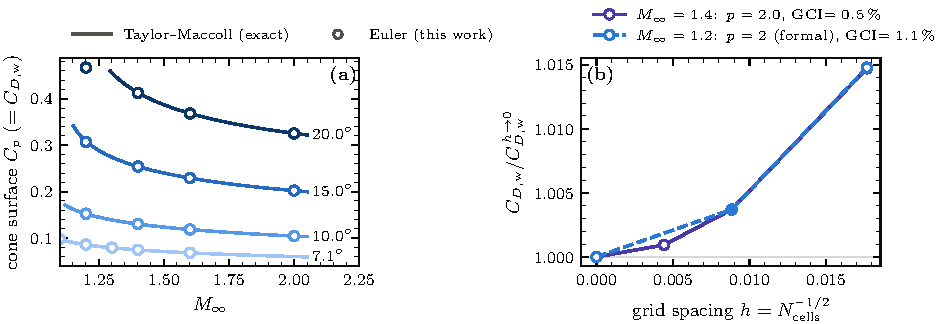
\includegraphics[width=\textwidth]{fig_validation}
\caption{(a) Cone surface pressure from the Euler solver (markers) against the exact
Taylor--Maccoll solution (lines). (b) Grid convergence of the nose wave drag, normalised by the
Richardson-extrapolated value (open: computed grids; filled: production grid).}
\label{fig:validation}
\end{figure}

\subsection{Transonic range}
\label{sec:transonic}

Steady Euler solutions converge too slowly below $M=1.1$ (detached shock far upstream, large
subsonic region), and RANS is needed there anyway because the shock interacts with the boundary
layer. The nose wave drag is therefore modelled as a smooth (cubic) rise from zero at $M=0.8$ to
the computed $M=1.1$ value at $M=1.0$, flat up to $M=1.1$. This assumption is common to all
shapes. The transonic Fluent runs listed in Section~\ref{sec:next} replace it.

\subsection{Flight model}
\label{sec:flight}

A point-mass trajectory is integrated from the \SI{12}{m} rail ($84^\circ$) to apogee. The drag
coefficient is built up from components (reference area $\pi D^2/4$):
\begin{equation}
C_D = k\left(C_{D,f} + C_{D,\rm fins} + C_{D,\rm base} + C_{D,e}\right) + C_{D,\rm w}(M),
\end{equation}
with turbulent, roughness-limited skin friction on the wetted area of nose and body (Schlichting,
compressibility-corrected), fin pressure drag (blunt leading edge subsonic, Ackeret hexagon
supersonic), the OpenRocket base-drag law (nozzle exit area removed while burning) and the ERT-Sim
excrescence law. The single factor $k$ is set so that the baseline nose (Von K\'arm\'an,
\SI{720}{mm}) reaches the LVO apogee of \SI{9.0}{km}. The resulting $M_{\max}=1.47$ is close to
the LVO's Mach 1.4 without further tuning. A longer nose adds its length to the vehicle and its
extra shell mass to the vehicle mass.

\subsection{Heating}
\label{sec:heating_method}

The wall cannot exceed the stagnation temperature $T_0=T_\infty(1+\tfrac{\gamma-1}{2}M^2)$, which
is the Firehorn design rule; the transient below shows how close it gets. At the tip, the laminar
stagnation-point coefficient (Fay--Riddell form without dissociation) with the modified-Newtonian
velocity gradient is
\begin{equation}
h_s = 0.763\,\mathrm{Pr}^{-0.6}\sqrt{\rho_s\mu_s \left.\frac{\mathrm du_e}{\mathrm dx}\right|_s}\;c_p,
\qquad
\left.\frac{\mathrm du_e}{\mathrm dx}\right|_s = \frac{1}{r_n}\sqrt{\frac{2(p_s-p_\infty)}{\rho_s}} ,
\end{equation}
so $h_s \propto r_n^{-1/2}$. Along the shell, the turbulent flat-plate correlation
$\mathrm{St}=0.0296\,\mathrm{Re}_x^{*-0.2}\mathrm{Pr}^{-2/3}$ (Eckert reference temperature) drives
the recovery temperature $T_r = T_\infty(1+r\tfrac{\gamma-1}{2}M^2)$, $r=\mathrm{Pr}^{1/3}$. The
wall response is a 1D transient conduction problem with an adiabatic inner face, which is
conservative because it neglects radiation and internal convection. Both are evaluated along the
nominal and the hot-day envelope trajectories.

\subsection{Stability, mass and payload}

Barrowman's method gives the nose $C_{N\alpha}=2$ at $x_{cp}=L-V/A_b$ and the fin contribution
($C_{N\alpha,f}=7.4$ for the assumed fins). The change in static margin relative to the baseline
nose is computed with positions measured from the aft end, including the CG shift from the
nose-shell mass. The shell mass is the wetted area times the Firehorn as-built areal density
(\SI{0.98}{kg/m^2}: \SI{500}{g} measured for the \SI{960}{mm}, \O\SI{240}{mm} nose). The 3U fit is
the length of curved nose over which $r\geq\SI{77}{mm}$.

\subsection{Design catalogue, robustness and CAD}

\begin{itemize}[leftmargin=*,itemsep=2pt]
\item \textbf{Direct runs at the design fineness.} All seven shapes (and the blunted Von K\'arm\'an
nose) were also computed at $L/D = 4.5$ for $M = 1.6$, 1.4 and 1.2. The full flow fields were saved
for the pressure maps of Section~\ref{sec:catalogue}.
\item \textbf{Robustness.} The apogee of every shape at $L/D = 4.5$ is recomputed with the onset of
the transonic drag rise moved to $M = 0.75$ and 0.85, the transonic wave drag scaled by
$\pm20\,\%$, the rest of the vehicle drag increased by 20\,\%, and the hot-day envelope with the LVO
masses.
\item \textbf{Renders and CAD.} The shaded views of Figure~\ref{fig:gallery} are computed from the
exact profiles (Lambert--Phong shading of the surface of revolution). The STL solids are
triangulated surfaces of revolution (128 azimuthal facets) closed by a flat base. Their
closure and outward normals were checked, and their volume matches the analytical one.
\end{itemize}
